\documentclass{kdo}

\usepackage[super]{nth}
\usepackage{url}
\usepackage{graphicx}
\usepackage{chants}

\begin{document}
% TODO:
% - write the section on the shape of a service
% - add instructions for tenken to come to the kokyo's side and when to leave.
% - add instructions for the sangha to stand during the morning service
% - add instructions for the kokyo to come to gassho during the chanting of the
%   ancestors.
% - paginate
% - proof
% - prohibit page breaks before \bline

\frontmatter
\begin{titlepage}
{\Huge\bf Kannon Do

  \bigskip\bigskip

 Regular Services}
\end{titlepage}

\begin{colophon}
Kannon Do Regular Services, Second Printing

\bigskip

\copyright\ 2015, Kannon Do Zen Meditation Center\\
1972 Rock Street, Mountain View, CA 94043\\
www.kannondo.org

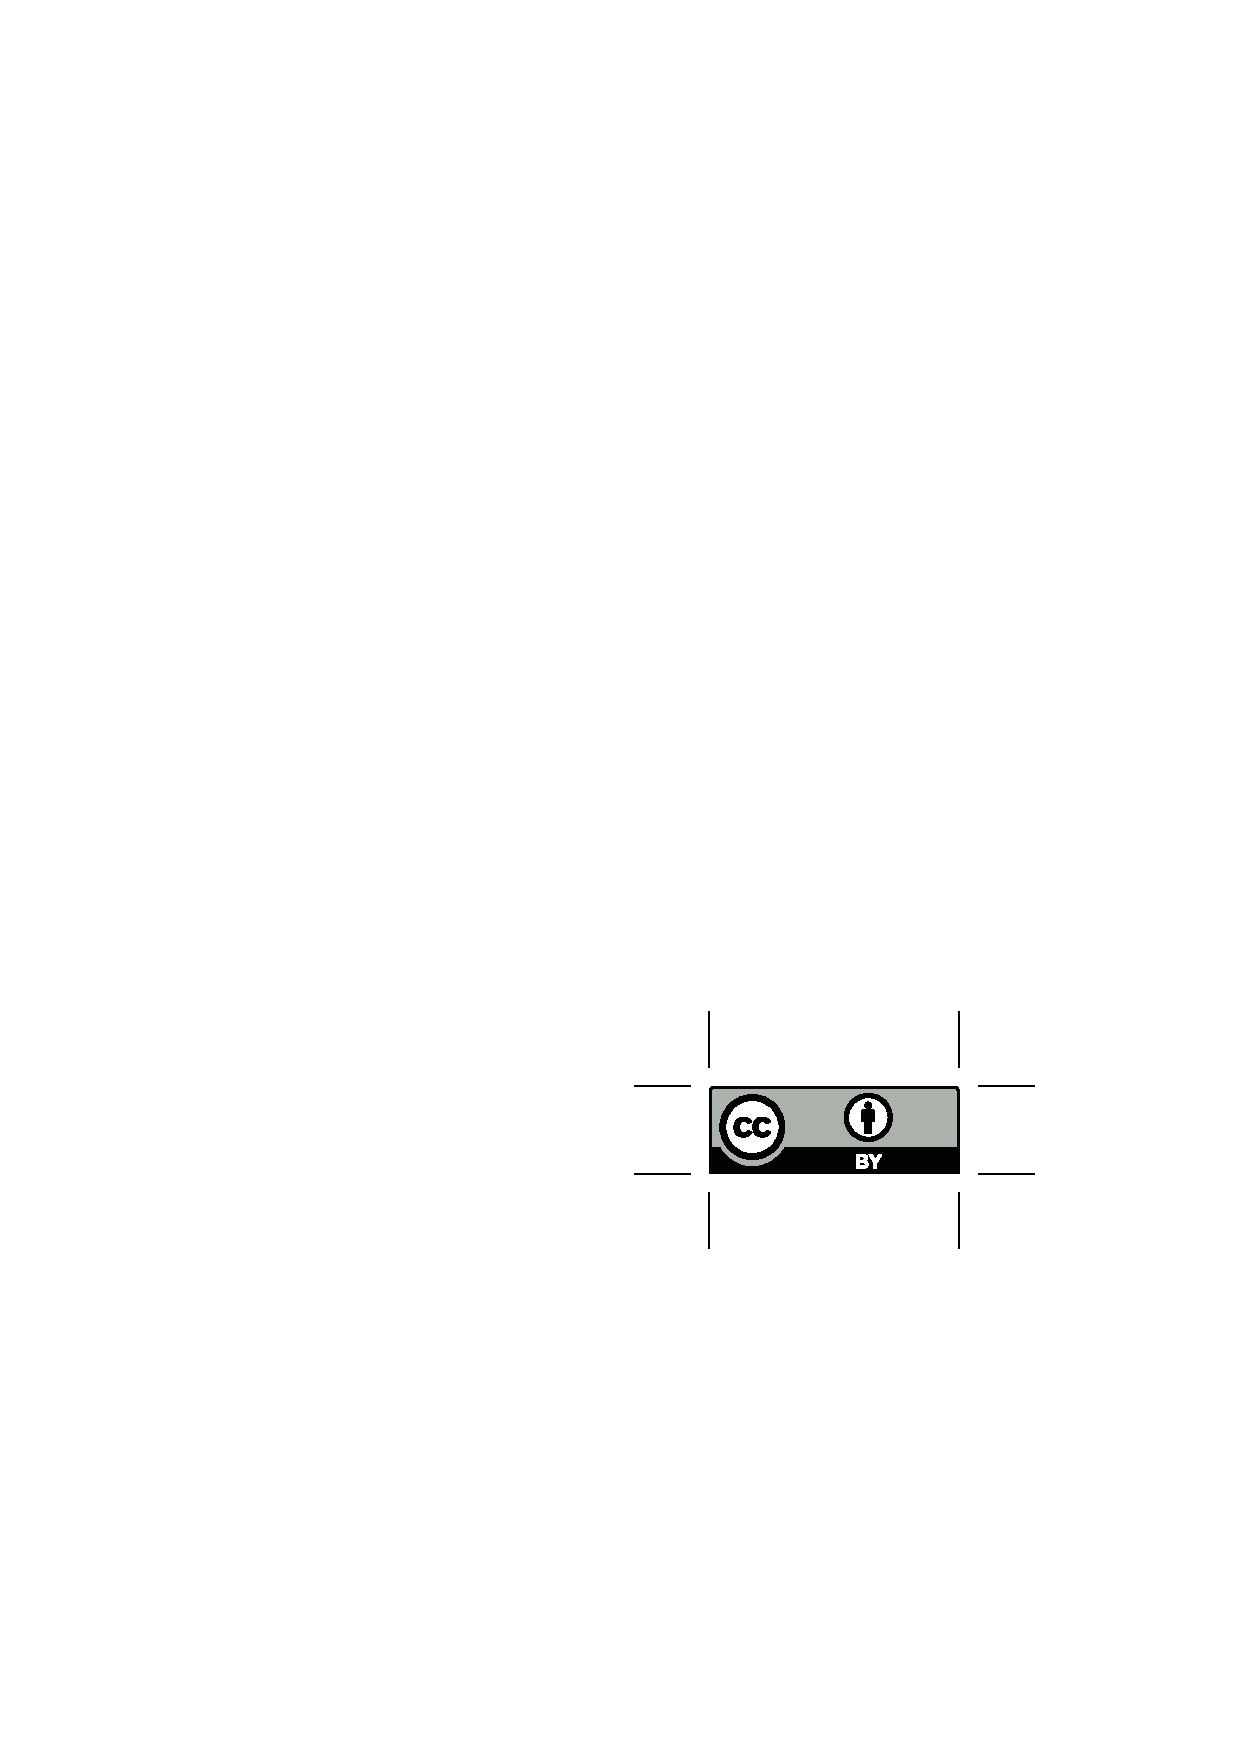
\includegraphics{by}

This work is licensed under the Creative Commons Attribution 4.0 International
License. To view a copy of this license, visit:\\
\url{http://creativecommons.org/licenses/by/4.0/}.

\bigskip

This book is set in 14\,pt.\ Fira Sans with \LaTeX\ and hand bound at Kannon Do.
\end{colophon}

\begin{dedication}
One thing flows into another\\
and cannot be grasped.\\
Before the rain stops, we hear a bird.

---Shunryu Suzuki
\end{dedication}

\cleardoublepage

\tableofcontents

\mainmatter

\chapter{Introduction}

\section{Service Positions}
\begin{description}
\item[Doshi] An ordained person who leads the service by offering incense and
leading prostrations and bows.
\item[Doan] Rings the bells.
\item[Tenken] Strikes the han (wooden block) to announce Wednesday evening
zazen, minds the lights, and opens the doors.
\item[Kokyo] Leads the chants during service.
\end{description}

\section{Explanation of Symbols}
The different bells are indicated by different symbols.

\subsection{Regular Rings of the Bells}

\begin{tabular}{llc}
Large Bell: & large red circle & \largebell \\
Small Bell: & small red dot & \smallbell \\
Zazen Bell: & small green diamond & \zazenbell
\end{tabular}

In addition to the regular rings, there are four sound effects that can be
produced on the large bell.

\subsection{Effects (\kern-.1ex Always on Large Bell)}
\begin{tabular}{llr}
Muffle: & red circle with $\times$ & \muffle \\
Bok: & red circle with slash & \bok \\
Clank: & red triangle & \clank
\end{tabular}

To produce a \muffle\ \emph{muffle}, hold the playing stick with two hands and
hold it firmly against the top of the bell to stop the ringing. Do not raise
the playing stick until the bell stops ringing. The playing stick should not
make a noise when it meets the top of the bell.

To produce a \bok\ \emph{bok}, hold the playing stick with two hands and bring
it down solidly against the top of the bell, then hold it in place. Do not
remove the playing stick until the bell has stopped ringing.

The difference between a bok and a muffle is whether the playing stick causes
the bell to ring when brought against the bell.

To produce a \clank\ \emph{clank}, grip the playing stick for the \emph{small
bell} like a pencil and bring the tip solidly against the side of the bell,
holding the playing stick against the bell until the bell stops ringing.

\section*{Doshi-Dependent Rings}
The timing of the second and third bell during long chants is determined by the
timing of the doshi's actions, as follows:

\begin{description}
\item[If the doshi goes up to offer incense.] The doshi will stand up and bow.
The doan rings the large bell as he bows. The doshi will go up to the altar and
offer chip incense, then will step back and bow to the altar. The doan rings
the bell as he bows.
\item[If the doshi stays sitting and puts hands in gassho.] Ring the bell as
the doshi's hands come up to gassho, and again as his hands come back down.
\end{description}

If the doshi does nothing, the doan does not ring the bells.

The approximate times to watch for the doshi's actions are indicated by
\doshidependent{blue text in italics.}

\section*{Using the Audio Equipment}
\subsection*{To turn on the audio equipment}
\begin{enumerate}
\item Press the red square button on the audio deck under the table. It will
light up and turn on the whole deck.
\item Bring up the master volume level toggle to the first rectangle.
\item Place the Lavalier next to the doshi's zabuton. Take care that the line
is neatly coiled and tucked under the clip.
\item Pick up the Sony Sound Recorder and turn it. The power button is on the
left side of the recorder. Pull down on the power button for 2 seconds.
\item Uncoil the headphone jacks under the cushions in front of the sound
table. Make sure the headphones are on the table for people to use if needed.
\item Take a seat on the zabuton on the floor next to the mixer. Once the
recorder is one, wait for the doshi to say ``Good evening,'' then hit the
record button. See the instruction sheet, ``Instructions for recording
lectures,'' sitting next to the mixer.
\end{enumerate}

\subsection*{At the end of the lecture}
When the doshi asks if there are any announcements, press the stop button on the
Sony Sound Recorder.

After the doshi concludes the service, open the zendo doors. Start with the
right one (if you are facing the altar) and then the left. Make sure they are
all the way open and the door catch has caught the door. The doshi and tenken
bow together syncronized with the doan bowing with the sangha.

After everyone has left the zendo, turn off the red power button on the mixer,
place the microphones in the bags, and place them below the sound table.

\begin{services}

\chapter{Zazen with Jundo}

\renewcommand{\footmark}{\bellkey}
\section*{At 5:30 AM}

\doan Prepare the altars by lighting the lamps.

Sit in the doan seat facing the bells and wait for the doshi.

\doshi Enter the zendo and perform a standing bow behind the mat. Walk around
the mat to the altar. Offer one long stick of incense, step back, and perform a
standing bow to the altar. Walk back around the bowing mat.

At the bowing mat, place bowing cloth on cushion, and perform three full bows.

\doan Ring the large bell once for each bow:
\jundoBows

\doshi Walk around the room in gassho.

Stand behind your cushion.

(If staying for zazen) put down bowing cloth and stick.

Bow to your cushion, turn and bow to the room, then sit down (or go to dokusan).

\doan Ring the zazen bell three times, evenly spaced, as the doshi bows:
\jundoStartZazen

Turn to face the wall.

\section*{40 minutes later}
\doan Ring the zazen bell once. \bigspace\zazenbell
\sangha Chant the robe chant.

\chapter{Regular Zazen}
\doan Prepare the altars by lighting the lamps.

Sit in the doan seat facing the bells and wait for the beginning of the period
of zazen.

\doan Ring the zazen bell three times, about 2 seconds apart:
\startZazenBells

Turn to face the wall.

\section*{40 minutes later}

\doan Ring the zazen bell once. \bigspace\zazenbell

\chapter{Kinhin}
\doan Ring the zazen bell twice at the end of zazen.
\kinhinBells

Carry the large inkin bell while doing kinhin.

\section*{10 minutes later}

\doan Ring the inkin bell once. \bigspace\zazenbell

\section*{Leaving the zendo}
\doshi Lead the sangha in a standing bow.
\tenken Open the zendo doors.
\doshi Exit the zendo, bowing.

(Outside) bow to the tenken.

\doan Lead the sangha in a shashu bow, synchronized with the doshi's bow to the
tenken.

Lead the sangha out of the zendo.

\chapter{Doan for Sesshin}
\subsection*{Silent Bowing}
\doan Stay seated in the doan seat, facing the bells.
\sangha Take your cushions to the center of the room, as on Saturday.
\doshi Offer incense, then lead the sangha in full bows.
\doan Ring the large bell once for every bow. \bigspace\largebell

At the end of 10 minutes, ring the large bell twice to signify the end of bows.

\bline{\hfill\largebell\hfill\largebell\hfill\null}

The ino or soku will seat everyone for the meal.

\part{Short Service, Wednesday Night}
\thumb{Wednesday Night}
\chapter{Wednesday Night}
\section*{At 7:00 PM}
\tenken Begin rolldown.
\doan Enter zendo, turn down overhead lights, light lamps on kaisando and main
altar.
\section*{At 7:10 PM}

\doshi Offer incense at the altar. Walk around bowing mat. Lay out stick,
bowing cloth, and papers. Bow to cushion. Turn and bow to the room. Sit down.

\doan Ring the zazen bell three times, evenly spaced, as the doshi bows.
\jundoStartZazen

\tenken Close the zendo doors and take your seat.

\section*{At 7:50 PM}
\doan Ring the zazen bell one time. \bigspace\zazenbell
\sangha Stand, fluff cushions, bow to cushions, bow to room. Face in to the
room.
\doan Get up and bow with the sangha. Take your seat again after the doshi
bows.
\doshi Lead the sangha in a standing bow.
\tenken Raise the lights.
\doshi Perform a standing bow behind the bowing mat, approach the altar and
offer one long stick of incense and two pinches of chip incense. Step back and
bow to the altar, then walk back around to the bowing mat and put out the
bowing cloth.

\pagebreak

\doan Ring the small bell as the doshi walks around the mat as follows:

\doshiBowingClothRolldown

The ringdown ends as the doshi drops the corners of the bowing cloth.

\kokyo Turn to face the altar as the doshi approaches it to offer incense.

\doshi Perform three full bows.

\doan Ring the large bell once for each bow. The first two rings are followed
by muffles as the doshi's hands touch down. The third is followed by a second
ring as his/her forehead touches down.
\firstBows

\sangha Bow with the doshi.

\doshi Approach the altar and offer more loose incense. Bow to the altar.
Return to the bowing mat.

\doan Ring the large bell once as the doshi bows to the altar, then ring the
small bell twice as the doshi passes the cushion.
\takeOutChantBookBells

\sangha Get out your chant books.

\kokyo Retrieve the kokyo's service book and stand to the right of the doan.

\tenken Retrieve the small mokugyo and stand to the right of the kokyo. Play the
mokugyo as the kokyo chants the words of the heart sutra.

\doshi Perform three full bows.

\doan Ring the large bell for the first two bows, and bok the bell on the
third.
\secondBows

\kokyo \heartOfGreatPerfectWisdomSutra

\kokyo May our intention equally extend to every being and place with the true
merit of Buddha's way $\sim$ \largebell

\allBuddhas*

\smallBellRolldown

\tenken Replace mokugyo and return to your cushion.
\kokyo Replace the kokyo's service book and return to your cushion.
\doan End the ringdown when everyone has put away their books.
\doshi Lead the sangha in three bows.
\doan Ring the small bell for each of the three bells, with a fourth ring as
the doshi's forehead touches the cushion on the third bow.
\lastBows

\doshi Pick up bowing cloth, stands behind mat. When the sangha is ready,
perform a standing bow toward the altar. Go to your cushion and bow to it. Turn
and bow to the room.

\doan Ring the small bell when the doshi bows toward the altar and the cushion.
When the doshi bows to the room, ring the bell twice, two seconds apart.
\beSeatedBells

\doshi Invite everyone to be seated.

\section*{Before Lecture}
\sangha Bring your cushions to the middle of the room.
\kokyo Serve speaker water, help with microphone and lectern as necessary,
then return to your seat.

\doshi Come to gassho.
\doan Bok the large bell: \bigspace\bok
\sangha \sutraOpeningVerse*
\newpage

\section*{After Lecture}
\doshi Come to gassho.
\doan Bok the large bell: \bigspace\bok
\sangha \fourVows*
\sangha Put away your cushions, stand in front of your place.
\doshi Lead everyone in a standing bow.
\tenken Open the zendo doors.
\doshi Exit the zendo, bowing.

(Outside) bow to the tenken.
\doan Lead the sangha in a shashu bow, synchronized with the doshi's bow to
the tenken.

Lead the sangha out of the zendo.

\part{Long Service, First and Third Saturday}
\thumb{\nth{1} \& \nth{3} Saturday}
\chapter{Long Service, First and Third Saturday}
\begin{service}
\kokyo \makaHannyaHaramittaShingyo
\pagebreak
\kokyo \enmeiJukkuKannonGyo
\kokyo \weDedicateThisMeritTo{Maka Hannya Haramitta Shin Gyo and the Enmei
Jukku Kannon Gyo for protecting life}
\sangha \allBuddhas*
\kokyo \songOfTheJewelMirrorSamadhi
\kokyo May we awaken Buddha's compassion and luminous mirror wisdom.

Chanting the Song of the Jewel Mirror Samadhi, we dedicate this merit and
virtue to: \bigspace\clank

\begin{outdent}
  \ancestorsShort*
\end{outdent}

\kokyo And to all the great women teachers, known and unknown, remembered
through these names: \bigspace\clank

\begin{outdent}
  \femaleAncestors*
\end{outdent}

\kokyo We dedicate our practice to all the great teachers from whom we have
received immeasurable benefit. And we venerate the founder of this temple,
great teacher Shogaku Shunryu. May our life reveal their compassion. Let us
honor their true being $\sim$ \largebell
\end{service}

\part{Long Service, Second and Fifth Saturday}
\thumb{\nth{2} \& \nth{5} Saturday}
\chapter{Long Service, Second and Fifth Saturday}

\begin{service}
\kokyo \makaHannyaHaramittaShingyo
\pagebreak
\kokyo \shosaimyoKichijoDharani
\kokyo \weDedicateThisMeritTo{Maka Hannya Haramitta Shin Gyo and the Shosaimyo
Kichijo Dharani for removing hindrance}
\sangha \allBuddhas*
\kokyo \harmonyOfDifferenceAndEquality
\kokyo May we awaken Buddha's compassion and luminous mirror wisdom. Chanting
the Harmony of Difference and Equality, we dedicate this merit and virtue to:

\begin{outdent}
  \ancestorsLong*
\end{outdent}

\kokyo Now we have dedicated our practice to the great teachers who have
transmitted the lamp through four countries. May our life reveal their
compassion. Let us honor their true being $\sim$ \largebell
\end{service}

\part{Service of Well Being, Fourth Saturday}
\thumb{\nth{4} Saturday}
\chapter{Service of Well Being, Fourth Saturday}
\begin{service}
\kokyo \makaHannyaHaramittaShingyo
\pagebreak
\kokyo \shosaimyoKichijoDharani
\kokyo \weDedicateThisMeritTo{the Maka Hannya Haramitta Shin Gyo and the
Shosaimyo Kichijo Dharani for removing hindrance}
\kokyo \lovingKindnessMeditation
\kokyo \enmeiJukkuKannonGyo
\kokyo May all awakened beings manifest through the three treasures their
luminous mirror wisdom. Having chanted the Loving Kindness Meditation and the
Enmei Jukku Kannon Gyo for protecting life, we dedicate its merit to

The benefit and well being of our great and abiding friends: \hrulefill

And to the benefit of all beings.\\
May they attain Buddha's Way. \largebell

\end{service}

\end{services}
\end{document}
